\documentclass{beamer}
\usepackage[utf8]{inputenc}

\usepackage{utopia} %font utopia imported
\usepackage{ amssymb }
\usepackage{enumerate}
\usepackage{graphicx}
\usetheme{Madrid}
\usecolortheme{default}
\usepackage{graphicx}
%------------------------------------------------------------
%This block of code defines the information to appear in the
%Title page
\title[Contrary-to-duty] %optional
{Contrary-to-duty reasoning, preference and violation}

\subtitle{About an obligation}

\author[Yingqin, Markus] % (optional)
{Yingqin Fu\inst{1} \and Markus Davydov\inst{2}}


\date[11.3. 2021] % (optional)
{11.03.2021}



%End of title page configuration block
%------------------------------------------------------------



%------------------------------------------------------------
%The next block of commands puts the table of contents at the 
%beginning of each section and highlights the current section:

\AtBeginSection[]
{
  \begin{frame}
    \frametitle{Table of Contents}
    \tableofcontents[currentsection]
  \end{frame}
}
%------------------------------------------------------------

\begin{document}
%The next statement creates the title page.
\frame{\titlepage}

%---------------------------------------------------------
%This block of code is for the table of contents after
%the title page
\begin{frame}
\frametitle{Table of Contents}
\tableofcontents
\end{frame}
%---------------------------------------------------------
\section{Introduction}
%---------------------------------------------------------
%Changing visivility of the text
\begin{frame}
\frametitle{Introduction}
\begin{description}
\item[$\bullet$]What is contrary-to-duty obligation?
\end{description}
\end{frame}
%---------------------------------------------------------
%Changing visivility of the text
\begin{frame}
\frametitle{Introduction}
What is contrary-to-duty obligation?
\begin{enumerate}
\item[$\bullet$] A contrary-to-duty obligation is an obligation telling us what ought to be the case if something forbidden is true.
\end{enumerate}
\begin{examples}
\begin{enumerate}
\item[$\bullet$] If she is guilty, she should confess
\item[$\bullet$] If he has hurt his friend, heshould apologise to her
\item[$\bullet$] If you are not going to keep your promise to him, you ought to call him
\item[$\bullet$] If the books are not returned by the due date, you must pay a fine
\end{enumerate}
\end{examples}
\end{frame}
%---------------------------------------------------------

\section{Chisholm's paradox}

%---------------------------------------------------------
%Highlighting text
\begin{frame}
\frametitle{Chisholm's paradox}

... known as one of the earliest CTD paradox.
Chisholm's paradox consists of the following four sentences:

\begin{block}{Chisholm's paradox}
\begin{enumerate}
\item  It ought to be that a certain man go to the assistance of his neighbours.
\item  It ought to be that if he does go, he tell them he is coming.
\item If he does not go then he ought not to tell them he is coming.
\item He does not go.
\end{enumerate}
\end{block}

\end{frame}
%---------------------------------------------------------
\begin{frame}{Chisholm’s paradox}
Chisholm’s paradox is a contrary-to-duty paradox, since it contains both a primary obligation to go, and a secondary obligation not to tell if the agent does not go.Yet intuitively the natural-language expressions
that make up the paradox are consistent and independent from each other: this is
why it is called a paradox.
    
\end{frame}

%---------------------------------------------------------
\section{Monadic deontic logic}
%---------------------------------------------------------
\begin{frame}{Monadic deontic logic}
\begin{enumerate}
\item[$\bullet$]Traditional or ‘standard’ deontic logic, often referred to as SDL
\item[$\bullet$]SDL regards as the most basic system of deontic logic
\item[$\bullet$]But also have the most drawbacks
\end{enumerate}
\end{frame}
%---------------------------------------------------------
\begin{frame}{Monadic deontic logic}
Quick overview about the Language, Semantics and Axioms
\begin{block}{Language}
\begin{enumerate}
\item[$\bullet$]$\varphi :=\perp | p |\neg \varphi |(\varphi \wedge \varphi)|\bigcirc\varphi|\square\varphi $\\
\item[$\bullet$]$\perp$:the empty symbol\\
\item[$\bullet$]$\neg$ $\varphi$: classical negation\\
\item[$\bullet$]$\varphi \vee  \phi $: classical disjunction\\
\item[$\bullet$]$\bigcirc \varphi $: $\varphi$ is obligatory\\
\item[$\bullet$]$ \neg \bigcirc\neg\varphi$: $ \varphi$ is forbidden\\
\item[$\bullet$]$ \square\varphi$: $\varphi$ is necessary
\end{enumerate}
\end{block}
\end{frame}
%---------------------------------------------------------
\begin{frame}{Monadic deontic logic}
Quick overview about the Language, Semantics and Axioms
\begin{block}{Semantics}
\begin{enumerate}
\item[$\bullet$ ]M, s $ \vDash $ p iff s $\in$ $\nu$  (p)
\item[$\bullet$ ]M, s $ \vDash $ $\neg \varphi$ iff not M, s $ \vDash $ $\varphi$
\item[$\bullet$ ]M, s $ \vDash $ $(\varphi\land\phi )$ iff M,s $ \vDash \varphi$ and  M,s $ \vDash \phi$
\item[$\bullet$ ]M, s $ \vDash  \bigcirc\varphi$ iff for all t,if Rst then M, t$\vDash \varphi$
\item[$\bullet$ ]M, s $ \vDash  \square\varphi$ iff for all t $\in$ W, M, t $\vDash \varphi$
\end{enumerate}
\end{block}
\end{frame}
%---------------------------------------------------------
\begin{frame}{Monadic deontic logic}
Quick overview about the Language, Semantics and Axioms
\begin{block}{Axioms}
\begin{enumerate}
\item Taut: All tautologies are Well formed formulas of the language.
\item  $Axiom K: O(p \to q) \to (O(p) \to O(q)) $
\item $ Axiom D: O(p) \to \neg O(\neg p)$
\item $Modus Ponens: ((p \to q) \land p) \to q $
\item $ Necessity: p \to O(p)$
\end{enumerate}
\end{block}
\end{frame}
%---------------------------------------------------------
\begin{frame}{The Limitations of SDL}
Now lets focus on the Chisholms paradox again.
\begin{block}{Chisholm's paradox}
\begin{enumerate}
\item  It ought to be that a certain man go to the assistance of his neighbours.
\item  It ought to be that if he does go, he tell them he is coming.
\item If he does not go then he ought not to tell them he is coming.
\item He does not go.
\end{enumerate}
\end{block}
\begin{block}{Chisholm's paradox in SDL}
\begin{enumerate}
\item $(1)O(h);(2)O(h\to t);(3)O(\neg h\to \neg t);(4) \neg h$
\item $(1)O(h);(2)O(h \to t);(3) \neg h \to O (\neg t); (4) \neg h$
\item $(1)O(h);(2)h\to O(t);(3)\neg h \to O(\neg t) ;(4)\neg h $
\item $ (1)O(h);(2)h\to O(t)(3)O(\neg h\to \neg t)(4)\neg h$
\end{enumerate}
\end{block}
\end{frame}
%---------------------------------------------------------
\begin{frame}{The Limitations of SDL}
\begin{block}{Chisholm's paradox in SDL}
\begin{enumerate}
\item $(1)O(h);(2)O(h\to t);(3)O(\neg h\to \neg t);(4) \neg h$
\item $(1)O(h);(2)O(h \to t);(3) \neg h \to O (\neg t); (4) \neg h$
\item $(1)O(h);(2)h\to O(t);(3)\neg h \to O(\neg t) ;(4)\neg h $
\item $ (1)O(h);(2)h\to O(t)(3)O(\neg h\to \neg t)(4)\neg h$
\end{enumerate}
\end{block}
\begin{enumerate}
\item From (4) and Axiom 5 ,we have $O(\neg h) $ ;From (1) and (2),we have O(t);From $O(\neg h)$ and (3),we have $ O(\neg t)$. Obviously,O(t) $\wedge$ $O(\neg t)$ is paradox.
\item From (3) and (4) with Axiom MP,we have $O(\neg t)$;From (2) and Axiom K,we have $O(h)\to O(t) $;which with (1) and Axiom MP,we have O(t)
\item We know that,$ \neg h \to (h \to O(t))$ is Taut,which with (4) can we have $ h \to O(t)$.it is identical to (2).Hence,it's redundant.
\item It's redundant with the same reason of 3.
\end{enumerate}
\end{frame}
%---------------------------------------------------------
\begin{frame}{The Limitations of SDL}
We can conclude:
\begin{enumerate}
\item[$\bullet$] Under the Monadic Deontic Logic(SDL) the CTD is inconsistent and redundant.
\item[$\bullet$] Something must be wrong with our formalisation, with SDL or with our intuitions.  
\end{enumerate}
Basically this puzzle is the contrary-to-duty (obligation) paradox.\newline\newline
So how can we overcome the limitation of SDL?Can we extend the semantics of SDL?
\end{frame}
%---------------------------------------------------------
\begin{frame}{The Limitations of SDL}
Yes for example, one can add distinct modal operators for primary and
secondary  obligations, where a secondary obligation is a kind of reparational obligation.\newline
So the sentences are now:
\begin{description}
\item[(1)] $\bigcirc_{1} h$
\item[(2)]$\bigcirc_{1}$ ($h \to t $)
\item[(3)]$\neg h \to \bigcirc_ {2} (\neg t)$
\item[(4)]$\neg h$
\end{description}
From 1-4 we can derive only $\bigcirc_{1} \neg t \wedge \bigcirc_{2} t$,which is consistent.\\
Seems like we find a good way to solve the limitation of SDL.However,it may not always be easy to distinguish primary from secondary obligations, because it may depend on the context whether an obligation is primary or secondary.
\end{frame}
%---------------------------------------------------------
\section{Dyadic deontic logic}
%---------------------------------------------------------
\begin{frame}{Dyadic deontic logic}
\begin{enumerate}
\item[$\bullet$]Also known as Dyadic Standart deontic logic
\item[$\bullet$]Logic for reasoning with dyadic obligations (“it ought to be the case that ... if it is the case that ...").
\item[$\bullet$]The language is extended with dyadic operators  $\bigcirc(p|q)$, which is true iff the preferred q worlds satisfy p.
\end{enumerate}
\end{frame}
%---------------------------------------------------------
\begin{frame}{Dyadic deontic logic}
Quick overview of the language and semantics
\begin{block}{Language}
\begin{enumerate}
\item[$\bullet$]$\varphi := \perp | p | \neg \varphi |(\varphi \wedge \varphi)|\square \varphi |\bigcirc(\varphi|\varphi)$\\
Given two arbitrary formulas $\phi$  and $\varphi$
\item[$\bullet$]...
\item[$\bullet$]$\bigcirc(\varphi\mid\phi$): It ought to be $\varphi$,given $\phi$\\
\item[$\bullet$]$P(\varphi\mid\phi) $:$\varphi$ is permitted,given $\phi$,as an abbreviation of $\neg\bigcirc(\neg\varphi\mid\phi)$\\
\item[$\bullet$]$\lozenge(\varphi)$:possibly $\varphi$,as an abbreviation of $\neg\square\neg\varphi$\\
\end{enumerate}
\end{block}
\begin{block}{Semantic}
\begin{enumerate}
\item[$\bullet$]...
\item[$\bullet$]M, s $ \vDash  \bigcirc(\phi\mid\varphi) iff \forall t(((M, t \vDash \varphi)\with\forall u(M, u \vDash \varphi) \Rightarrow t \geq u) \Rightarrow M, t \vDash \phi)$
\item[$\bullet$]M, s $ \vDash  \square\varphi$ iff for all t $\in$ W, M, t $\vDash \varphi$
\end{enumerate}
\end{block}

\end{frame}
%---------------------------------------------------------
\begin{frame}{Limitations of DSDL}
\begin{block}{A variant of the Chilsom's paradox}
\begin{enumerate}
\item[A]It ought to be that Jones does not eat fast food for dinner.
\item[B]It ought to be that if Jones does not eat fast food for dinner, then he does not go to McDonald’s.
\item[C] If Jones eats fast food for dinner, then he ought to go to McDonald’s.
\item[D]Jones eats fast food for dinner.
\end{enumerate}
\end{block}
\end{frame}
%---------------------------------------------------------
\begin{frame}{Limitations of DSDL}
\begin{block}{A variant of the Chilsom's paradox}
\begin{enumerate}
\item[A]It ought to be that Jones does not eat fast food for dinner.
\item[B]It ought to be that if Jones does not eat fast food for dinner, then he does not go to McDonald’s.
\item[C] If Jones eats fast food for dinner, then he ought to go to McDonald’s.
\item[D]Jones eats fast food for dinner.
\end{enumerate}
\end{block}
\begin{block}{A variant of the Chilsom's paradox in DSDL}
f:Jones eats fastfood for dinner; m:he goes to McDonald’s 
\begin{enumerate}
\item[A]$\bigcirc \neg f$
\item[B]$\bigcirc(\neg m \mid \neg f)$
\item[C]$\bigcirc(m\mid f)$
\item[D]f
\end{enumerate}
\end{block}
\end{frame}
%---------------------------------------------------------
\begin{frame}{Limitations of DSDL}
\begin{block}{A variant of the Chilsom's paradox in DSDL}
f:Jones eats fastfood for dinner; m:he goes to McDonald’s 
\begin{enumerate}
\item[A]$\bigcirc \neg f$
\item[B]$\bigcirc(\neg m \mid \neg f)$
\item[C]$\bigcirc(m\mid f)$
\item[D]f
\end{enumerate}
\end{block}
\\
The dyadic representation A - D highlights the dilemma between factual detach-ment (FD) and deontic detachment (DD)
\begin{description}
\item[Axiom FD]$\bigcirc(m\mid f),f \Rightarrow \bigcirc m$\\
\item[Axiom DD]$\bigcirc(\neg m \mid \neg f), \bigcirc\neg f \Rightarrow \bigcirc\neg m$\\
\end{description}
\end{frame}
%---------------------------------------------------------
\begin{frame}{Limitations of DSDL}
From A and B wit axiom DD ,we have $\bigcirc\neg  m$;From C and D(axiom FD),we have $\bigcirc m$ , as we simply derive a dilemma:$\bigcirc\neg m\wedge\bigcirc m$\\
Hence,there is also something wrong with the DSDL,when we try to reasoning CTD paradox.\\
The main drawback of DSDL is that in a monotonic setting, we cannot detach
the obligation $\bigcirc m$ from the four sentences.

\end{frame}
%---------------------------------------------------------
\section{Input/Output logic}
\begin{frame}
\frametitle{Input/Output logic}
\begin{enumerate}
\item[$\bullet$]  Input/Output logic is a non classical logic
\item[$\bullet$]  they may be expressed in terms like: In such-and-such a situation, so-and-so should be the case, or …should be brought about, or …should be worked towards, or …should be followed.
\item[$\bullet$]Input/output logic may be seen as an attempt to extract the essential mathematical structure behind the reconstruction of deontic logic.
\end{enumerate}

\end{frame}
%---------------------------------------------------------
\begin{frame}{Input/Output logic}
\begin{block}{Definition}
\begin{enumerate}
    \item Cn(A)  denotes  the  set  of  logical  consequences  of  A  in  classical  propositionallogic.It returns the set of all provable propositional formulae provable assumingthe fact in A( the set of answers of a set of inputs).
    \item G(A) is the set of answers of a set of inputs.
\end{enumerate}
\end{block}
\begin{examples}
A= \{ x, y\} then Cn(A) = \{x, y, x $\vee $y, x $\wedge$ y $\vee$ . . . \}
\end{examples}
\begin{examples}
G1 = \{(a1, x1),(a2, x2)\} and A1\{a1, z\} and A2 = \{a1, a2, x2\}\\
G1(A1) = {x1}\\
G1(A2) = {x1, x2}
\end{examples}

    
\end{frame}
%-----------------------------------------------------------

\begin{frame}{Rules}
What's more,there are 5  rules in I/O logic:
\begin{enumerate}

\item[$\bullet$] Strengthening Input (SI): From (a,x) to (b,x) whenever a $\in$ Cn(b)
\item[$\bullet$] Conjoining Output (AND): From (a,x), (a,y) to (a,x$\wedge$y)
\item[$\bullet$] Weakening Output (WO): From (a,x) to (a,y) whenever y $\in$ Cn(x).
\item[$\bullet$] Disjoining input (OR): From (a,x), (b,x) to (a$\vee$b,x)
\item[$\bullet$] Cumulative transitivity (CT): From (a,x), (a$\wedge$x,y) to (a,y).
\end{enumerate}
    
\end{frame}
%------------------------------------------------------------
\begin{frame}{Systems of input/output}
There are also four very natural systems of input/output, which are labelled as follows: 
\begin{description}
\item[$\bullet$]simple-minded alias $out_{1}$(G,A) = Cn(G(Cn(A)))
\item[$\bullet$]basic (simple-minded plus input disjunction: $out_{2}$)
\item[$\bullet$]reusable (simple-minded plus reusability: $out_{3}$)
\item[$\bullet$]reusable basic alias $out_{4}$
\end{description}
 For example,$out_{4}$ can be given by Figure 2.   
\end{frame}
%----------------------------------------------------------
\begin{frame}{systems of input/output}
\begin{figure}
\centering
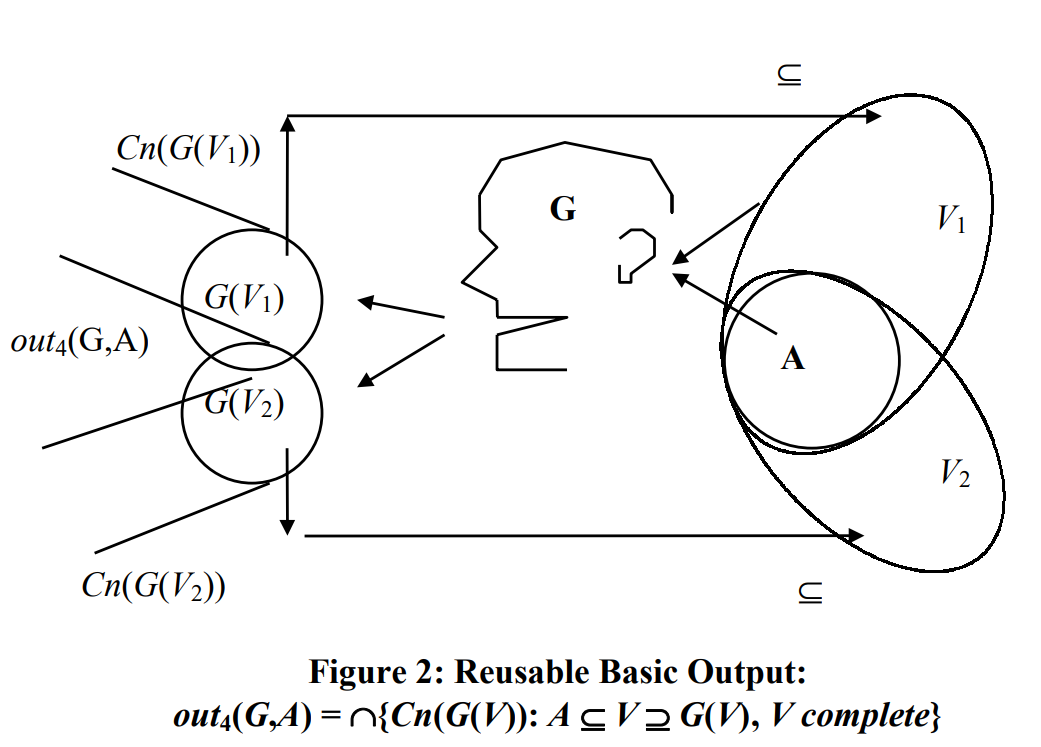
\includegraphics[scale=0.3]{out4.png}

\label{fig_framework}
\end{figure}
\end{frame}
%------------------------------------------------------------
\begin{frame}{Contrary to duty reasoning}
\begin{block}{Definition(Maxfamilies)}
Let G be a set of conditional norms and A and C two sets of propositional formulas.\\
Then maxfamily(G, A, C) is the set of maximal
subsets H $\subseteq$ G such that out(H, A) $\cup$ C is consistent.(which means,out(H,A)) is consistent with C.)\\

\end{block}
For a possible solution to Chisholm’s paradox, consider the following output operation $out^{\cap}$:\\
$out^{\cap}(G, A) = \cap
\{out(H, A) | H \in maxfamily(G, A, A)\}
$
    
\end{frame}
%--------------------------------------------------------------
\begin{frame}{Contrary to duty reasoning}
Let G a "Chisholm norm set";\\
x means the norm that a man goes to the assistence of his neighbors;\\
z means the norm that he tells them he is coming\\
\begin{enumerate}
\item[$\bullet$]G=$\{(\top ,x),(x,z),(\neg x,\neg z)  \}$
 , $(\top ,x)$ means the norm that the man must go to the assistance of his neighbors;$(x,z)$means the norm that it ought to be that if he goes he ought to tell them he is coming;$(\neg x,\neg z)$ means that the norm that if he does not go he ought not to tell them he is coming.
 \item[$\bullet$] $A=\{ \neg x \}$
 \item[$\bullet$] We have H $\in out_{1}(G,A)=\{x,\neg z\}$ ,which is inconsistent with A because of $\top$
 \item[$\bullet$] We have  H = maxfamily(G,A,A)=$ \{ G\setminus \{(\top,x) \}\}=\{\{(x,z),(\neg x,\neg z)   \}\} $
 \item[$\bullet$] out(H,A)=$\neg z$,which is consistent with A
 \item[$\bullet$]$out^{\cap}(G,A)=Cn(\neg z)$ ,which means the form that the man must not tell his neighbors he is coming.
\end{enumerate}
\end{frame}
%-------------------------------------------------------------------
\section{Counterfactual Deontic Logic}
\begin{frame}{Counterfactual Deontic Logic}
Counterfactual Deontic Logic,which is introduced by Rönnedal in 2016.The Counterfactual Deontic Logic combine the Counterfactual Logic with Deontic Logic.It aims at the relationship between the obligation and time.
\begin{block}{Definition}
\begin{enumerate}
  \item[$\bullet$]$A\square \rightarrow B$ is often read ‘If A were the case, then B would be the case’
\item[$\bullet$]R is a temporal operator; ‘$Rt_{1}$A’ says that it is realised at time t1 (it is true at t1) that A
\end{enumerate}
\end{block}
\end{frame}
%---------------------------------------------------------------
 \begin{frame}{Contrary to duty reasoning}
 Consider the following sentences about Contrary to duty paradox
\begin{enumerate}
\item[1] (On Monday it is true that) You ought to keep your promise (and see your friend on Friday).
\item[2] (On Monday it is true that) It ought to be that if you keep your promise, you do not apologise (when you meet your friend on Saturday).
\item[3](On Monday it is true that) If you do not keep your promise (i.e. if you do not see your friend on Friday and help her out), you ought to apologise (when you meet her on Saturday).
\item[4](On Monday it is true that) You do not keep your promise (on Friday).
\end{enumerate}
     
 \end{frame}
 %----------------------------------------------------------------------------
 \begin{frame}{Contrary to duty reasoning}
 With the help of Counterfactual Deontic Logic,the four sentences can now be symbolised in the following way:(R is a temporal operator;t1,t2,t3 are the different time;k is keep promise;and a is apologise )
\begin{enumerate}
\item[CF1]$Rt_{1}ORt_{2}k$
\item[CF2]$Rt_{1}O(Rt_{2}k \square \rightarrow Rt_{3}\neg a)$
\item[CF3]$Rt_{1}(Rt_{2}\neg k \square \rightarrow Rt_{2}ORt_{3}a)$
\item[CF4]$Rt_{1}Rt_{2}\neg k$
\end{enumerate}
 \end{frame}
 %-------------------------------------------------------------------------
 \begin{frame}{Contrary to duty reasoning}
 \begin{enumerate}
\item[$\bullet$] CF-CTD is consistent,It does not seem to be possible to deduce any contradiction from the four sentences. Hence, we want our symbolisation of this set to be consistent. In this respect, CF-CTD is an intuitively plausible formalisation of the four sentences.
\item[$\bullet$] CF-CTD is non-redundant.There ist no sentence in this set follows from the rest.

\end{enumerate}    
\begin{block}{Limitations}
The Counterfactual Deontic Logic seems to be a proposed solution of CTD-paradox(at least in our example).However,it also has limitations.\\
\begin{enumerate}
\item[$\bullet$]the Counterfactual Solution cannot Handle Timeless (or Parallel)
Contrary-to-Duty Paradoxes;
\item[$\bullet$]the Counterfactual Solution cannot Solve Beforehand
Contrary-to-Duty Paradoxes
\end{enumerate}
\end{block}
\end{frame}
%----------------------------------------------------------------------
\section{Alternative approaches}
\begin{frame}{Alternative approaches}
\begin{block}{approach 1}
 Carmo and Jones suggest that the representation of the facts is challenging,
instead of the representation of the norms. In their approach, depending on the
formalisation of the facts various obligations can be detached.
\end{block}
\begin{block}{approach 2}
A recent representation of Chisholm'paradox is to replace deonitc detachment by so-called aggregative deontic detachment(ADD),and to derive from A-D the obligation  $(\neg f \wedge \neg m)$and m, but not $\neg $m.\\
$\bigcirc (m|f),f \Rightarrow \bigcirc m $ FD\\
$\bigcirc(\neg m |\neg f),\bigcirc\neg f \Rightarrow \bigcirc(\neg m \wedge \neg f)$ ADD\\
The limitation of this approaches is that we can no longer accept the principle of weakening(also known as inheritance). 
$\bigcirc(\neg m \wedge\neg f|\top) \Rightarrow \bigcirc(\neg m |\top)$
\end{block} 
\end{frame}
%---------------------------------------------------------------------------
\section{Conclusion}
\begin{frame}{Conclusion}
Accordingly, CTDs are the source for many paradoxes and the driver for the
development of many formalisms and deontic logics.In our opinion,the key point of CTD Paradoxs  is that how can we find a adequate formel to deal with the relationship between \textbf{obligation} and \textbf{condition}.
\end{frame}
%---------------------------------------------------------------------------
\begin{frame}{Example}
Consider the sentence from section 3:
\begin{enumerate}
\item[B] It ought to be that if Jones does not eat fast food for dinner, then he does not go to McDonald’s.
\end{enumerate}
which can be formed as:
\begin{enumerate}
\item[$\bullet $]$\bigcirc (\neg f \rightarrow\neg m)$
\end{enumerate}

However, in our opinion,"if Jones does not eat fast food for dinner "is a \textbf{condition} (instead of obligation) of "he ought to not go to McDonald's".We cannot lump these two concepts together.
So the better form should be:
\begin{enumerate}
\item[$\bullet$]$ \neg f \rightarrow \bigcirc \neg m$
\end{enumerate}
However,this is also redundant due to $f \vDash\neg f \rightarrow \bigcirc \neg m $
\end{frame}
%-------------------------------------------------------------------------------------
\begin{frame}{Conclusion}
We always find a limitation,when we try to form CTD with deontic logic,especially SDL.More and more approaches are proposed.Many researchers also build the binary deontic logic to solve them......When a new deontic logic is proposed, the traditional contrary-to-duty examples are always the first benchmark examples to be checked,which is always the biggest challenge of DL System.What's more,it is also a challenge for our own moral life and law system.\\
Perhaps there is not an eternal solution to solve the paradoxes entirely.But with the research on all the challenges for multiagent deontic logic,the law system will be more and more perfect,our obligation and violation will be more and more clearly... 
\end{frame}
\end{document}